
\documentclass[letterpaper, 10 pt, conference]{IEEEtran}
%\usepackage[dvips]{graphicx}
    \usepackage[pdftex]{graphicx}
    \graphicspath{{../pdf/}{../jpeg/}}
    \DeclareGraphicsExtensions{.pdf,.jpeg,.png}



\usepackage[cmex10]{amsmath}
\usepackage{amssymb}
\usepackage{mathrsfs}
\usepackage{bm}
\usepackage{dsfont}
%\usepackage[pdftex]{graphicx}
% \usepackage[dvips]{graphicx}

\usepackage{graphicx}
\usepackage{subfigure}
\graphicspath{ {images/} }
\usepackage{cite}
\usepackage{bibentry}
%\usepackage[dvips]{color}
%\usepackage{lipsum}
\usepackage{mathtools}
\usepackage{cuted}
\usepackage{xfrac}
\usepackage{multirow}
\usepackage{arydshln}






% correct bad hyphenation here
\graphicspath{{37SP/}{37SP_C/}{tolcon_4_SP/}{tolcon_37_SP/}{tolcon_123_SP/}
{tolcon_4_3f/}{tolcon_37_3f/}{tolcon_123_3f/} {MC_4_SP/}{123SP/}{123SP_C/}{4_SP_TRX/} {4_SP_Power/}
{4_3f_trx/}{4_3f_Power/}{37_3f_clasic/}{37_3f_trx/}{123_3f_clasic/}{123_3f_trx/}{8500reduced_PF/}{8500reducedvar_PF/}}
\hyphenation{op-tical net-works semi-conduc-tor}


\begin{document}
\title{Optimal coordination of directional earth fault overcurrent relays  67N in interconnected electric power systems}
% Economic optimization of transmission tower grounding and insulation
%
%
% author names and IEEE memberships
% note positions of commas and nonbreaking spaces ( ~ ) LaTeX will not break
% a structure at a ~ so this keeps an author's name from being broken across
% two lines.
% use \thanks{} to gain access to the first footnote area
% a separate \thanks must be used for each paragraph as LaTeX2e's \thanks
% was not built to handle multiple paragraphs
%

\author{ P.~M.~De~Oliveira-De Jesus$^{1}$~\IEEEmembership{Senior Member,~IEEE}, E.~Sorrentino$^{2}$, J.~S.~Abello$^{1}$, O.~Archilla$^{1}$, C.~A.~Alza$^{1}$ \\, D.~Celeita$^{1}$\IEEEmembership{Senior Member,~IEEE}, G.~A.~Ramos~$^{1}$\IEEEmembership{Senior Member,~IEEE} A.~J.~Urdaneta~$^{3}$\IEEEmembership{Senior Member,~IEEE}
\IEEEauthorblockA{\\$^1$ Universidad de los Andes, Bogot\'a, Colombia.
\\ $^2$ Universidad Carlos III, Madrid, Spain. \\
$^3$ Universidad Simon Bolivar, Caracas, Venezuela.
}}
%\thanks{Manuscript received November XX, 20XX}
%\thanks{J.~S.~Abello, O.~Archilla, C.~A.~Alza, D.~Celeita, G.~A.~Ramos, and P.\,M.\,De Oliveira-De Jesus are with the Department of Electrical and Electronic Engineering, Universidad de Los Andes, Bogot\'a, Colombia. E-mail: pm.deoliveiradejes@uniandes.edu.co.  A.~J.~Urdaneta is with Simon Bolivar University, Venezuela.
%E-mail: alberto@usb.ve, E.~Sorrentino is with Carlos III University, Madrid, Spain.
%E-mail: elmersor@usb.ve} % <-this % stops a space
%       \thanks{Digital Object Identifier}}

\markboth{Transactions on Power Delivery,~Vol.~X, No.~X, March~2020}%
{De Oliveira-De Jesus: Transactions on Power Delivery}
\maketitle
\begin{abstract}
In this paper, the classic optimization model applied to coordinate 67 directional overcurrent relays in interconnected systems is applied to coordinate 67N neutral directional overcurrent relays. To do so, single-phase to neutral short-circuit currents are determined using the multiphase-multiground (4-wire) network model developed by EPRI for the OpenDSS platform. The OpenDSS network model is based on primitive impedances. This model overcomes the limitations of symmetrical components by including the effect of unbalanced loads, systems with different X/R ratios, neutral grounding through earth resistances and fault impedances
 on short-circuit currents passing through all relays of the system. As a key contribution, we investigate the impact of high-impedance single-phase to neutral/earth faults in the  optimal clearing times and selectivity of the protection system. The results show the optimal operation time decreases as the fault impedance increases until the calculated time dial setting stagnates at the minimum value. Beyond this point, the clearing times reach a minimum and deteriorate as far the fault impedance increases.
\end{abstract}


\begin{IEEEkeywords}
directional overcurrent relays coordination, high-impedance faults,  single phase faults
\end{IEEEkeywords}

\IEEEpeerreviewmaketitle

%\section*{Nomencalture}
%
%\begin{IEEEdescription}[\IEEEusemathlabelsep\IEEEsetlabelwidth{${CFO}_k$}]
%%\item[ $\mu_i$]  Annual frequency of flashes cloud-to-ground intercepted by section/tower $k$ in flashes/100km-yr
%\item[ $\eta_k$]  Expected ground flash density at section/tower $k$ in flashes/km$^2$-year
%\item[ $\w^b_k$]  Basic insulator length specified for switching surges/60Hz at section/tower $k$ in cm
%\item[ $\w_k$]  Insulator length at section/tower $k$ in cm
%\item[ $\Delta \w_k$]  Additional Insulator length at section/tower $k$ in cm
%\item[ $\sigma_{Gk}$]  Incremental tower cost for increasing insulator length in all phases of section/tower $k$ in $\$$/cm
%\item[ $C_{Gk}$]  Additional insulation costs at section/tower $k$ in $\$$
%%\item[ $\rho_{i1}$]  First-layer earth resistivity in $\Omega$-m
%%\item[ $\rho_{i2}$]  Second-layer earth resistivity in $\Omega$-m
%%\item[ $\lambda_i$] Expected ground flash density $\lambda_i$ at section $S_i$ in flashes/km$^2$-year
%%\item[ $A$] Terminal substation A
%%\item[ $B$] Terminal substation B
%%\item[ $b_i$]  Distance between ground wires of tower $i$ in m
%%\item[$C_{ij}^G$]  Installation cost of scheme $u_{ij}^G$, electrode ${G}_j$ at tower $i$, in $\$$
%%\item[$C_{ik}^I$]  Installation cost of scheme $u_{ik}^I$, insulation ${CFO}_k$ at tower $i$, in $\$$
%%\item[$\boldsymbol{CFO}$]  Set of available insulation levels
%%\item[${CFO}_{k}$]  Critical Flashover Overvoltage $k$ in kV
%%\item[$\boldsymbol{C^I}$]  Set of insulation level costs
%%\item[$\boldsymbol{C^G}$]  Set of grounding electrode costs
%%\item[ $d_{i1}$]  Depth of first resistivity layer in m
%%\item[$\boldsymbol{G}$]  Set of available grounding electrode schemes
%%\item[${G}_j$]  Tower footing electrode scheme $j$
%%\item[ $h^s_i$]  Average height of the shield wires in m
%%%\item[ $h^l_i$]  Average height of the phase wires in m
%%\item[ $H_i$]  Line altitude of tower $i$ in meters over the sea level
%%\item[ $I_{ijk}$] Critical flashover current in kA
%%\item[ $L_i$] Section length of tower $i$ in m
%%\item[ $L_T$] Total line length in m
%%\item[ $l_C$]  Counterpoise length in m
%%\item[ $l_B$]  Ground bar length in m
%%\item[$N_G$]  Number of available electrode schemes
%%\item[$N_I$]  Number of available insulation levels $k$
%%\item[$N_T$]  Number of towers along the line
%%\item[ $p_{ijk}$] Probability that peak stroke current in any flash will exceed  the critical back-flashover current $I_{ijk}$
%%\item[$P_i$]  Atmospheric pressure of tower $i$ in mmHg
%%\item[$R_{ij}$]  Impulse resistance of the tower footing in $\Omega$
%%\item[ $S_i$] Section or area covered by tower $i$ in m$^2$
%%\item[ $T_a^i$]  Annual average air temperature at section $S_i$ in Celsius degrees
%%\item[$T$]  Outage rate in tripouts/100km-year
%%\item[ $T_{ijk}$] Outage rate of tower $i$ with grounding electrode $j$ and insulation level type $k$ in tripouts/100km-year
%%\item[ $T^{max}$] Maximum admissible line outage rate in tripouts/100km-year
%%\item[$\boldsymbol{U}$] Set of electrode and insulation schemes.
%%\item[$\boldsymbol{u}^G$] Set of grounding electrode schemes.
%%\item[$\boldsymbol{u}^I$] Set of insulation schemes.
%%\item[$u_{ij}^G$] Grounding electrode scheme $j$  at tower $i$
%%\item[$u_{ik}^I$]  Insulation scheme $k$  at tower $i$
%%\item[$V_{ik}$] Corrected Insulation level at tower $i$ in kV.
%%\item[$V_i^T$] Ground potential rise at tower $i$ in kV.
%%\item[$V_n$] Line-to-ground operational voltage in kV.
%%\item[ $W_i$] Width of section $i$ in m.
%%\item[ $x_{ijk}$] Binary decision variable (0,1) associated to the installation of insulation level type $k$ and grounding electrode type $j$ and at tower $i$
%%\item[ $\boldsymbol{x}$] Set of specified decision variables.
%%\item[ $x_i,y_i,z_i$]  GG_0raphical coordinates of tower $i$ in m
%%\item[ $Z^i$]  Impedances of phases and shield wires of tower $i$ in $\Omega$
%%\item[  ]  Sub-indexes
%%\item[$i$]  Identifies tower $i$
%%\item[$j$] Identifies  electrode scheme $j$
%%\item[$k$]  Identifies insulation scheme $k$
%\end{IEEEdescription}

%The calculation of this type of overvoltages must be carried out with many uncertainties, given the random nature of the lightning and the imprecise knowledge of its main parameters.

\section{Introduction}

In 1988, \cite{urdaneta1988} presented a linear-programming  approach to solve coordination problem of directional overcurrent relays (DOCR) in interconnected systems. The original method was applied to coordinate function 67 considering three-phase to ground faults. Thus, optimal relay settings are determined according to a set of feasible current magnitudes based on solid three-phase to ground short-circuits \cite{ezzeddine2011coordination}. Since then, a large number of contributions have been proposed to tackle the classical optimal coordination problem resorting to different optimization procedures focusing on the 67 function. Recent and comprehensive reviews of existing optimization procedures can be found in \cite{hussain2013optimal, 7753935, emerald, 6880088}.

However, we can observe from above-mentioned review papers that no contributions are devoted to the optimal coordination of 67N functions in interconnected systems. The 67N function  is widely applied in sub-transmission systems to detect single and two phase to ground faults and to provide backup to the distance residual function 21N.

Over the last decade, this topic has gained renewed interest since under the smart grid paradigm, medium voltage sub-transmission and distribution networks are being operated under weakly-meshed schemes in order to improve the power system reliability. So, traditional radial-based operation supported in unidirectional overcurrent protection relays are not longer suitable. The use of directional overcurrent relays to protect meshed networks might be a cost effective alternative.

As the function 67N has not been duly considered  we need to determine the magnitude of the asymmetrical faults seen by the 67N function to setup the optimization procedure. A fundamental shortcoming of the short current calculation lies on the use of traditional sequence models disregarding important effects such as mutual couplings, current division at neutral/grounding path and the effect of high-impedance faults. On account of the existence of several short-circuit calculation tools based on multiphase-multiground network models such as the OpenDSS \cite{opendss}, it is now possible to determine precisely how different fault impedance magnitudes change the fault currents and therefore the response of the protection system whose settings were setup assuming fault currents associated with solid faults.

The effect of high impedance faults are critical to ensure speed and selectivity. The magnitude of the fault impedance is of stochastic nature. The coordination problem of 67N relays must account that many faults are not solid. Existing optimization procedures cannot answer how high-impedance single-phase to neutral faults affect the optimal clearing time, the selectivity and, the corresponding optimal relay settings. This aspect has been overlooked in literature.

To fulfill the research gap, this paper updates the original optimal model to coordinate DOCR \cite{urdaneta1988} considering  67N relays and investigating how different magnitudes of high-impedance faults affect the quality of the optimization results, i.e. the optimal clearing times as well as the selectivity and the sensitivity of the protection system. To do so, the proposal is illustrated with the well-known three bus test system introduced by \cite{urdaneta1988} redefined now as a multiphase-mutiground network system.


The paper is organized as follows. Section \ref{theoptmodel} describes the method used. The case-study is defined in Section \ref{casestudy}. Results are discussed in Section \ref{results}. Conclusions are drawn in Section \ref{conclusions}.


\section{Method} \label{theoptmodel}



The original optimization problem was written to coordinate  67 phase relays considering solid three-phase faults \cite{urdaneta1988}. This method is now adapted to perform optimal coordination of 67N relays in meshed systems when different fault impedances (not only solid faults) occurs in the system affecting speed and selectivity.

\subsection{Assumptions}

Real-wold power systems are complex and for the sake of simplicity the following assumptions and limitations are considered in the formulation of the optimization problem.


\begin{enumerate}

\item The optimization problem is posed by assuming that the magnitude of the fault impedance is the same for all possible "relevant" faults, just as the standard model \cite{urdaneta1988} assumes that all relevant faults are solid, that is $R_F$=0. The use of a unique fault impedance magnitude for all faults of the model is debatable in account of its stochastic nature. It is clear that the coordination problem must be solved for the expected fault impedance magnitude and the corresponding variances. However, if we account the fault impedance magnitude as a probability function, the approach turns the model into a stochastic optimization problem. The stochastic view of this problem is matter of further research.


\item All asymmetrical phase-to-neutral faults were produced at same phase. In this case we select phase $c$ (the nearest to ground).

\item Transient configurations are not included in the optimization problem formulation. In real-world the relaying system does not operate at the same time. Thus, the short circuit current magnitude seen by each relay adopts different values owing to topology changes. Despite this problem has been solved in \cite{urdaneta1997optimal,sorrentino2020novel}, this aspect has been overlooked in all existing DOCR optimization. The main consequence of disregard transient configurations lies on increased sensitivity problems in backup relays due to unrealistic low fault currents.

   \item The use of the OpenDSS tool to determine fault currents include prefault conditions. However. in this paper we neglect load currents, neither balanced nor balanced.

   \item We assume that the sensitivity problem is solved. In this paper we assume all relays are adjusted with the same pick-up currents of the 67N function. In general this value is set between 10 \% of the current transformer capacity and 80 \% of minimum short circuit current.

  \item Short-circuit current magnitudes are assumed as invariant values over time. The effect of decrement factors are not included.

  \item Only time-delayed relays are considered.  The coordination time is unique for all primary-backup pairs. The effect of time-definite adjusts are out of scope.

\item Circuit breaker operation times are not included in the model.

  \item Only IEC standard curves are considered, and all the relays are assumed to be with the same curve.

  \item Equivalent impedances at source buses are assumed the same at peak and off-peak load. Thus, the fault currents do not change along the time.

\item Resistance of all ground mats at substations are equal to zero.

\item The optimization model is built considering that near-end and far-end Faults occur at substations.

\item Influence of stability constraints is not considered.

\item Once the optimization model is defined, a sensitivity analysis is performed considering a range of fault impedance magnitudes from 0 to a maximum value when the optimization problem becomes not well-defined and therefore unsolvable.
\end{enumerate}




 
 
 
\subsection{Problem formulation}

 Consider a meshed power system with $k$=1,...,$n_l$ three-phase transmission lines. The set of transmission lines is defined as $k\in \mathds{N}$ with $n_l=\dim{(\mathds{N})}$. Each line has two overcurrent 67N relays. Thus, a  total of $r$=1,$\ldots$, $n_r$=2$n_l$ relays are installed in the system. The set of relays is defined as $r\in \mathds{R}$ with $n_r=\dim{(\mathds{R})}$. Each relay  $r\in \mathbf{R}$ is characterized by the following manner. Current-time curve parameters for each relay are fixed and defined by three parameters: $\alpha_{r1}\in \bm {\alpha}$,  $\alpha_{r2}\in \bm {\alpha}$ and $\alpha_{r3}\in \bm {\alpha}$. Pick-up currents $P_r \in \bm {P}$
 depend on maximum unbalanced currents that may flow by the line, and  the time dial setting $D_r\in \bm {D}$ are defined by the protection engineer according to a coordination criteria.
\begin{figure}[t] \centerline{
     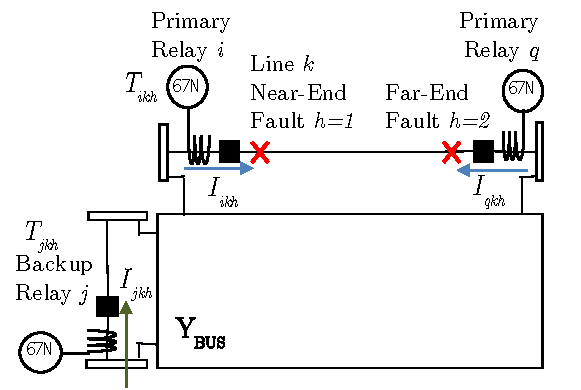
\includegraphics[width=2.3in]{images/main-backup.pdf}}
       \caption{Primary-backup relays}
      \label{main}
        \end{figure}

Figure \ref{main} shows a faulted line $k\in \mathbf{N}$. Line $k$ is protected by two primary  67N overcurrent relays $i\in \mathds{R}$ and $q\in \mathds{R}$. Depending on the network topology, we can identify a number of relays pairs (primary relay $i\in \mathds{R}$ and backup relay $j\in \mathds{R}$) that must be coordinated.
The set of relevant faults is defined as $h\in \mathds{H}$ with $n_f=\dim{(\mathds{H})}$ the number of faults under consideration. We identify two relevant faults per line $k$, $\mathds{H}$=$\{1,2\}$. Thus, $n_f$=2. A near-end fault ($h$=1) whose location is closer to relay $i$ and a near-far fault ($h$=2) adjacent to relay $q$. Given a fault $h\in \mathds{H}$ over the line $k$, if a primary relay $i$ does not clear the fault, another adjacent (backup) relay $j$ (located in other adjacent line) should clear the fault. All relays of the system can operate as primary or backup depending on whether the fault is located in its own line or the fault is located in adjacent line.


Figure \ref{main} shows the situation when both primary relays $i$ and $q$  operate successfully when a fault $h$ occurs in line $k$. In this case, each primary-backup relay-pair $i-j$ must fulfill the following inequality time operation constraint:


\begin{equation} \label{SCTstat}
  T_{jkh}-T_{ikh}\geq C\quad i,j\in \mathds{R}, k\in \mathds{N}, h\in \mathds{H}
\end{equation}

where $T_{ikh}$ is a primary  operating time (for a relay $i$ located in the line $k$ with fault $h$),  $T_{jkh}$ is a backup operating time (for a relay $j$ located in an adjacent line of the line $k$ with fault $h$, not in the same line), and $C$ is a known value, the coordination time specified by the protection engineer for all primary-backup pairs.





The operation time for the primary relay $i$ when the fault $h$ occurs at line $k$ is expressed as:

\begin{equation}\label{primary}
  T_{ikh}=\frac{\alpha_{i1} D_{i}}{(\frac{I_{ikh}}{P_{i}})^{\alpha_{i2}}+\alpha_{i3}}=\beta_{ikh}D_{i}
\end{equation}

where single-phase short-circuit current contribution seen by a relay $i$ due to fault $h$ at line $k$ ($I_{ikh}$) must be determined using the primitive admittance matrix $Y_{BUS}$ with all breakers of the system closed. The maximum multiplier allowed is $M^{max}$=$\frac{I_{ikh}}{P_{i}}$=30. For short-circuit $I_{ikh}$ currents higher than $30{P_{i}}$, the operation time is constant  $T_{ikh}$=$\frac{\alpha_{i1} D_{i}}{30^{\alpha_{i2}}+\alpha_{i3}}$.

Likewise, the  operation time for the backup relay $j$ when the fault $h$ occurs at line $k$ is expressed as:

\begin{equation}\label{primaryxx}
  T_{jkh}=\frac{\alpha_{j1} D_{j}}{(\frac{I_{jkh}}{P_{j}})^{\alpha_{j2}}+\alpha_{j3}}=\beta_{jkh}D_{j}
\end{equation}

where single-phase short-circuit current contribution seen by a relay $j$ due to fault $h$ at line $k$ ($I_{jkh}$) must be determined using the primitive admittance matrix $Y_{BUS}$ with all breakers of the system closed. Thus, given a fault $h$ at line $k$ both adjacent relay operation times can be expressed as a function of relay curve parameters and pick-up currents. Primary operation time  $T_{ikh}$=$\beta_{ikh}D_{i}$ where $\beta_{ikh}$=${\alpha^{-1}_{i1}}{[(\frac{I_{ikh}}{P_{i}})^{\alpha_{i2}}+\alpha_{i3}]}$ must be lower than the backup operation time $T_{jkh}$=$\beta_{jk}D_{j}$ where $\beta_{jkh}$=${\alpha^{-1}_{j1}}{[(\frac{I_{jkh}}{P_{j}})^{\alpha_{j2}}+\alpha_{j3}]}$. Therefore, Eq. \ref{SCTstat} can be rewritten as:

 \begin{equation} \label{SCTstat2}
  \beta_{jkh}D_{j}-\beta_{ikh}D_{i}\geq C\quad  i,j\in \mathds{R}, k\in \mathds{N}, \mathds{H}=\{1,2\}
\end{equation}

where $C$ is the predefined coordination time. Normal load and short circuit currents are sensed by neutral directional overcurrent functions 67N through the sum of three phase currents measured by current transformers at phases or a by  a separate current transformer for grounded neutrals at each substation.

Linear factors $\beta_{ikh}$ and  $\beta_{jkh}$   should be determined considering two feasible single-phase faults located at near-end ($h$=1) and far-end of line $k$=1,...,$n_l$. It is important to stress out that  $\beta_{ikh}$  factors depend on single-phase to neutral short circuit magnitudes $I_{ikh}$  whose magnitudes are strongly dependent upon the grounding path. As a result, $I_{ikh}$ can be determined using a detailed network model such as EPRI's NEV OpenDSS platform.

Optimization problem constraints can be now defined for a generalized system with $n_l$ lines, $n_r$ relays and $n_f$=2 feasible fault locations. According to Equations \ref{SCTstat2}, \ref{SCTtran} and \ref{eles}, a total of $n_b$ feasible primary-backup pair constraints must be identified and grouped in this compact form:

\begin{equation}\label{BB}
 \mathbf{B}\cdot\mathbf{D}\ge C\mathbf{u}
\end{equation}

where  $\mathbf{D}$ is the $n_r$ dimension vector with the time dial of each relay and $\mathbf{B}$ is the   coordination matrix that depends on linear factors $\beta_{ikh}$  and $\beta_{jkh}$ for $h$=1,2. The coordination matrix $\mathbf{B}$ has $n_r$ columns and $n_b$ rows. The number of rows will depend on the number of effective primary-backup pairs. Entry  $\mathbf{u}$ is a $n_b$ row unit vector and $C$ is the specified coordination time between primary and backup relays.

The objective function (OF) of the optimization problem is defined as the average sum of operating times of all the
primary relays for the two faults ($n_f$=2), near-end and far-end faults under consideration:

\begin{equation}\label{objective}
  \mbox{OF}=\frac{1}{n_f}\sum_{h=1}^{n_f}\sum_{k=1}^{n_l}\sum_{i=1}^{n_r}m_{ik}  T_{ikh}
\end{equation}


where $m_{ik}$ is equal to 1 if the primary relay $i$ is located at line $k$, otherwise  $m_{ik}$=0.


Finally, once the objective function and the corresponding constraints are duly defined, the optimization problem is stated as follows.
For a given the system data (primitive admittance matrix) and relay data (current-time parameters and pickup currents) determine the best set of time dial settings ($\mathbf{D^*}$) that minimizes the overall system primary relay operation time (OF) considering selectivity constraints.

\begin{eqnarray}\label{odocr1}
& &  \min_{\mathbf{D^*}} \quad \mbox{OF}=\frac{1}{n_f}\sum_{h=1}^{n_f}\sum_{k=1}^{n_l}\sum_{i=1}^{n_r}m_{ik}  T_{ikh}  \\ \nonumber
& & \mbox{subject to}:\\\label{odocr2}
& &\mathbf{B}\cdot\mathbf{D}\ge C\mathbf{u}\\\label{odocr3}
& &\mathbf{D}\le\mathbf{D^{max}}\\\label{odocr4}
& &\mathbf{D}\ge\mathbf{D^{min}}
\end{eqnarray}

where  $\mathbf{D^{min}}$ and $\mathbf{D^{max}}$ are the dial limits vectors.
The optimization problem has $n_r$ unknowns. The maximum number of inequality restrictions will be 4$n_l$ if all pairs primary-backup relays are able to detect the magnitude and/or direction of the fault.
The above stated optimization problem is suitable to be solved using any linear programming tool, such as Matlab's LinProg.


In this paper, we investigate how the objective function ($OF$) and the optimal settings ($\mathbf{D}$) are affected when the coordination matrix ($\mathbf{B}$) is calculated using different high-impedance phase to neutral fault conditions. To do so, single-phase short-circuit currents $I_{ikh}$ and $I_{jkh}$ are calculated using a multiphase-multiground model considering different fault resistances $R_f$.

 \section{Test system}  \label{casestudy}

\begin{figure}[t!] \centerline{
     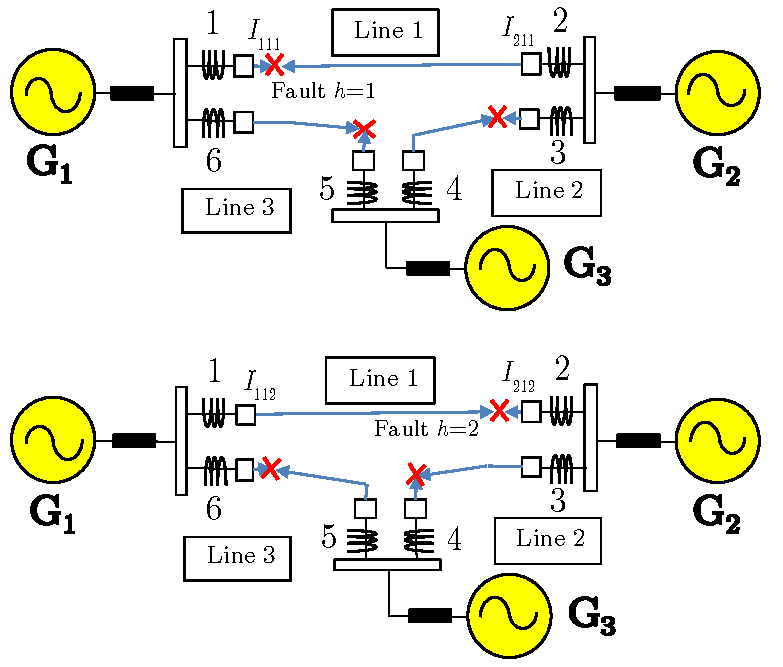
\includegraphics[width=6.4cm]{images/figure1.pdf}}
       \caption{Test system - One-line diagram and fault locations\cite{urdaneta1988}}
      \label{figure1}
        \end{figure}

                 \begin{figure*}[t!] \centerline{
     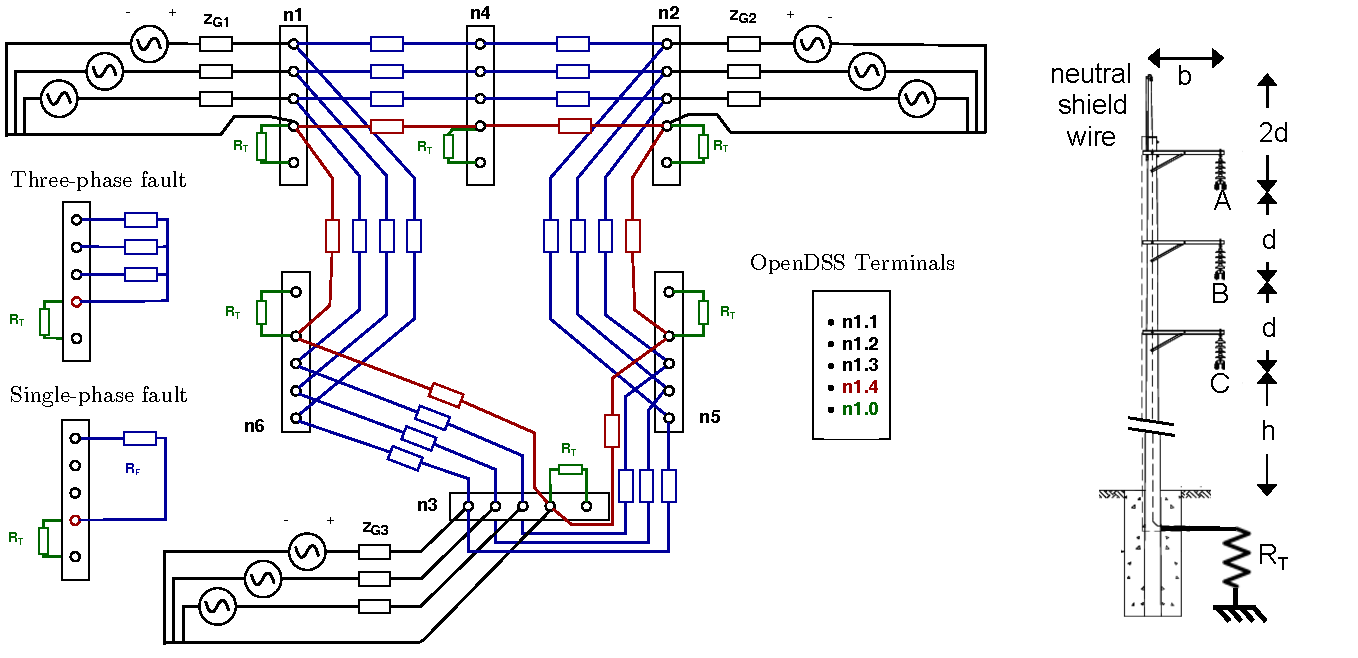
\includegraphics[width=12.0cm]{images/figure2.pdf}}
       \caption{Test system - Multi-phase Multi-ground diagram}
      \label{figure2}
        \end{figure*}



The classic formulation was originally applied over the test-system depicted in Fig. \ref{figure1} considering three-phase faults and the coordination of six relays 67P.
The original test system comprises three substations, three generators with reactance $X^+_1$ = $X^-_1$ = $X^0_1$ = 20  \% (100 MVA), $X^+_2$ = $X^-_2$ = $X^0_2$ = 12 \% (25 MVA) and $X^+_3$ = $X^-_3$ = $X^0_3$ = 18 \% (50 MVA). Positive sequence series impedance of the three lines are:
 $Z^+_1$ = 5.5 + j 22.85 $\Omega$ (50km), $Z^+_2$ = 4.4 + j 18.00 $\Omega$ (40km) and $Z^+_3$ = 7.6 + j 27.00 $\Omega$ (60km). The system has no loads.
  67N phase relay parameters are $\alpha_{i1}$ = 0.14, $\alpha_{i2}$ = 0.02, $\alpha_{i3}$ = -1 for $i$ = 1,...,6 (IEC standard inverse curve). All pick-up currents were set 50A.

Positive sequence impedance parameters for lines and generators are given above in order to determine three-phase short-circuit currents required by  67 (phase) relays to operate. However, in order investigate how to optimize the coordination of  67N (neutral) relays we need to determine exact short-circuit currents for single phase $c$ to neutral faults. To do so, we must build an equivalent 4-wire model for the original positive sequence model provided in \cite{urdaneta1988}  by scripting a new multi-phase multi-ground model under the OpenDSS platform \cite{opendss}.

Figure \ref{figure2} shows the multiphase diagram equivalent for the one-line diagram depicted in Fig. \ref{figure1}. The OpenDSS tool provides an explicit network representation for all system elements.
Besides  three-phases represented in blue color, system neutrals (shield wires) and ground resistances $R_T$ are highlighted in red color and green colors, respectively. Single-phase to neutral faults are represented by $R_F$. For instance, a single-phase $c$ to neutral fault with $R_F$=100 $\Omega$ in line 1 is coded as: \scriptsize
 \texttt{New fault.1   Bus1= n4.3   Bus2=n4.4 r=100}. \normalsize


Primitive impedance matrices  for lines and generators must be provided. Transmission lines primitive matrices are get from the tower sketch shown in Fig. \ref{figure3} with dimensions provided in Table \ref{Table2}. Phase conductor characteristics are given in
Table  \ref{Table3}. Transmission line positive sequence impedances for the tower structure depicted in   Fig. \ref{figure3} coincides with the ones specified in the original three-bus test case \cite{urdaneta1988}.

     \begin{figure}[t!] \centerline{
     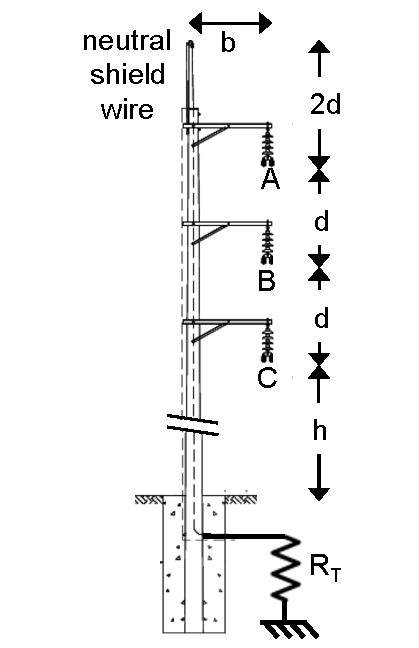
\includegraphics[width=3.0cm]{images/figure3.pdf}}
       \caption{Test system - 69kV tower sketch}
      \label{figure3}
        \end{figure}


\begin{table}[b]
\begin{center}\caption{Tower/pole geometry sketch}\label{Table2}
\centering
\begin{tabular}{lccccc}\hline
Line & $d$ (ft)  & $b$ (ft) & $h$ (ft) & Phase conductor & Neutral  \\\hline
1-2  & 7.85 & 6.0      &  40 & 500MCM Conlay AA & ACSR 4/0 6/1\\
2-3  & 9.70 & 5.0      &  40 & 605MCM 54/7 ACSR & ACSR 4/0 6/1\\
3-1  & 10.6 & 5.5      &  40 & 605MCM 54/7 ACSR & ACSR 4/0 6/1\\\hline
\end{tabular}
\end{center}
\end{table}

\begin{table}[b]
\begin{center}\caption{Phase \& neutral conductor characteristics}\label{Table3}
\centering
\begin{tabular}{lccc}\hline
Type & Size & Resistance (ohm/mile)  & GMR (ft)  \\\hline
ACSR 6/1 & 4/0 AWG  & 0.5920 & 0.00814 \\
AA Conlay & 500 MCM & 0.2023 & 0.02600 \\
ACSR 54/7 &605 MCM&0.1756 &0.03210\\\hline
\end{tabular}
\end{center}
\end{table}


The case-study shown in Fig. \ref{figure2} has six buses. Buses 1, 2 and 3 correspond to generating substations and buses 4, 5 and 6 correspond to a faulted point at given distance from substation $k$, for $k$=1,2,3. In this paper, we only use near-end and near-far faults as seen in  Fig. \ref{figure1}. Thus, the distance of all faults from substations is set equal to 1 meter.


The six bus system depicted in  \ref{figure2} was scripted in OpenDSS. Short-circuit impedances of generators are provided under a three-phase base coinciding with the original ones.




  \section{Results}  \label{results}

The problem solution approach is described in detail so that the interested reader can easily replicate the results with the script included in the following GitHub page: https://github.com/pmdeoliveiradejesus/Optimal-67N-DOCR-coordination. All Simulations were performed in Matlab with the LinProg optimization tool. Fault currents were acquired from the OpenDSS using the COM interface. Specific cases were also coded and solved with MS Excel's solver tool for illustrative purposes.


  The proposed optimization model was applied to the case-study described in Section \ref{casestudy}.
    The case study has $n_l$ = 3, $\mathds{N}$=\{1,2,3\}, lines and $n_r$ = 6 relays,
      $\mathds{R}$=\{1,2,3,4,5,6\}. Two faults ($n_f$=2) are modelled.


      Two scenarios are analyzed:
\begin{enumerate}
  \item Case 1: Faults at near-end and far-end of all lines with $R_F$=0 $\Omega$
  \item Case 2: Faults at near-end and far-end of all lines with $R_F$=10.0 $\Omega$
\end{enumerate}

Finally a sensitivity analysis is carried out varying $R_F$  from 0  $\Omega$ to 50  $\Omega$  when the optimization problem becomes not-well defined due to low currents make the relay system insensible.

A total of $n_b$ = 12 primary-backup ($ikh$-$jkh$) pairs are identified. The fault currents ($I_{ikh}$ and $I_{jkh}$) determined using the OpenDSS 4-wire model and the corresponding $\beta$-factors ($\beta_{ikh}$ and $\beta_{jkh}$) for both scenarios are listed in Tables \ref{kappas} and \ref{kappas2}.


  \begin{table*}[h!]\centering\label{kappas}
\begin{tabular}{ccc|ccc|cc|cc|c|c}\hline
 \multicolumn{3}{c|}{primary}  &  \multicolumn{3}{|c|}{backup}  &  \multicolumn{2}{|c|}{$I_{ikh}$}
  &  \multicolumn{2}{|c|}{$I_{jkh}$} & $\beta_{ikh} $  &  $\beta_{jkh}$\\\hline
$i$ &   $k$&    $h$     &  $i$ &   $k$&    $h$     & kA & deg & kA & deg & & \\\hline
1	&	1	&	1	&	5	&	1	&	1	&	5.1084	&	31.3988	&	0.4562	&	42.5829	&	1.9889	&	3.0967	\\	
3	&	2	&	1	&	1	&	2	&	1	&	2.8496	&	33.1075	&	0.6687	&	42.3876	&	1.9889	&	2.6299	\\	
5	&	3	&	1	&	3	&	3	&	1	&	3.4665	&	32.6495	&	0.6777	&	41.3936	&	1.9889	&	2.6161	\\	
2	&	1	&	1	&	4	&	1	&	1	&	0.5215	&	41.1806	&	0.0461	&	46.7550	&	2.9161	&	-85.9869	\\	
4	&	2	&	1	&	6	&	2	&	1	&	0.7424	&	41.4553	&	0.0624	&	52.2838	&	2.5252	&	31.4513	\\	
6	&	3	&	1	&	2	&	3	&	1	&	0.5327	&	43.7341	&	0.1097	&	-130.3178	&	2.8892	&	8.8425	\\	
1	&	1	&	2	&	5	&	1	&	2	&	0.6688	&	42.3873	&	0.0614	&	-128.0885	&	2.6298	&	34.0328	\\	
3	&	2	&	2	&	1	&	2	&	2	&	0.6777	&	41.3932	&	0.1107	&	49.8779	&	2.6160	&	8.7418	\\	
5	&	3	&	2	&	3	&	3	&	2	&	0.4563	&	42.5825	&	0.0453	&	-133.6871	&	3.0964	&	-70.9221	\\	
2	&	1	&	2	&	4	&	1	&	2	&	2.9246	&	33.1159	&	0.7424	&	41.4557	&	1.9889	&	2.5253	\\	
4	&	2	&	2	&	6	&	2	&	2	&	3.3188	&	32.6413	&	0.5326	&	43.7344	&	1.9889	&	2.8893	\\	
6	&	3	&	2	&	2	&	3	&	2	&	5.1749	&	31.3988	&	0.5214	&	41.1812	&	1.9889	&	2.9163	\\	

\hline
  \end{tabular}
  \caption{Case 1 - Linear Factors and Short-circuit currents (low impedance faults)}
\end{table*}

  \begin{table*}[hbt!]\centering\label{kappas2}
\begin{tabular}{ccc|ccc|cc|cc|c|c}\hline
 \multicolumn{3}{c|}{primary}  &  \multicolumn{3}{|c|}{backup}  &  \multicolumn{2}{|c|}{$I_{ikh}$}
  &  \multicolumn{2}{|c|}{$I_{jkh}$} & $\beta_{ikh} $  &  $\beta_{jkh}$\\\hline
$i$ &   $k$&    $h$     &  $i$ &   $k$&    $h$     & kA & deg & kA & deg & & \\\hline
1	&	1	&	1	&	5	&	1	&	1	&	2.9041	&	84.4839	&	0.2595	&	95.6736	&	1.9889	&	4.1810	\\	
3	&	2	&	1	&	1	&	2	&	1	&	2.0375	&	72.8356	&	0.4783	&	82.1258	&	1.9889	&	3.0303	\\	
5	&	3	&	1	&	3	&	3	&	1	&	2.3696	&	75.5376	&	0.4633	&	84.2914	&	1.9889	&	3.0746	\\	
2	&	1	&	1	&	4	&	1	&	1	&	0.2966	&	94.2584	&	0.0264	&	99.8622	&	3.8622	&	-11.0201	\\	
4	&	2	&	1	&	6	&	2	&	1	&	0.5310	&	81.1846	&	0.0449	&	92.0539	&	2.8933	&	-64.5410	\\	
6	&	3	&	1	&	2	&	3	&	1	&	0.3643	&	86.6348	&	0.0748	&	-87.4114	&	3.4550	&	17.2953	\\	
1	&	1	&	2	&	5	&	1	&	2	&	0.4784	&	82.1255	&	0.0437	&	-88.3691	&	3.0301	&	-52.3010	\\	
3	&	2	&	2	&	1	&	2	&	2	&	0.4634	&	84.2910	&	0.0759	&	92.7831	&	3.0744	&	16.7195	\\	
5	&	3	&	2	&	3	&	3	&	2	&	0.2596	&	95.6732	&	0.0256	&	-80.6462	&	4.1805	&	-10.5220	\\	
2	&	1	&	2	&	4	&	1	&	2	&	2.0912	&	72.8295	&	0.5309	&	81.1849	&	1.9889	&	2.8934	\\	
4	&	2	&	2	&	6	&	2	&	2	&	2.2687	&	75.5255	&	0.3643	&	86.6350	&	1.9889	&	3.4552	\\	
6	&	3	&	2	&	2	&	3	&	2	&	2.9418	&	84.4878	&	0.0354	&	94.2615	&	1.9889	&	3.8626	\\		
	\hline
  \end{tabular}
  \caption{Case 2 - Linear Factors and Short-circuit currents (high.impedance faults)}
\end{table*}

Notice that some primary-backup ($ikh$-$jkh$) pairs have currents with opposite directions (631-231,
112-512,  532-332). In case 1 and case 2 some  $\beta$-factors
are negative. This means the existence of short-circuit contributions lower
that the selected pick-up currents (50A).  In case 1 all short-circuit contributions are greater
that the selected pick-up currents except primary-backup ($ikh$-$jkh$) pairs 211-411 and 112-512.
In  case 2, primary-backup ($ikh$-$jkh$) pairs 211-411,
421-621,631-231 do not operate for near-end faults and relay pairs 112-512, 322-122, 532-332 do not operate for far-end faults. It is clear that as in case 2 $R_F$ is not solid some loss of sensitivity is observed.

  The general optimization model is given by the minimization of sum of all primary times when the fault occurs at near-end and near-far of each line of the system constrained to the coordination equation and corresponding time delay setting limits as follows:

\scriptsize

\begin{equation}\label{Bm}
   \min_{\mathbf{D^*}}\quad \beta_{111}D_1+\beta_{212}D_2+\beta_{321}D_3+\beta_{422}D_4+\beta_{531}D_5+\beta_{632}D_6
\end{equation}


\begin{eqnarray}   \label{opt2}
&&\mbox{subject to}:\\\nonumber
&&  \begin{bmatrix}
    -\beta_{111}    &   0   &   0   &   0   &   \beta_{511} &   0   \\
    \beta_{121} &   0       &   -\beta_{321}    &   0   &   0   &   0   \\
  0&  0       &   \beta_{331} &   0   &   -\beta_{531}    &   0   \\
  0&  -\beta_{211}        &   0   &   \beta_{411} &   0   &   0   \\
0&  0       &   0   &   -\beta_{421}    &   0   &   \beta_{621} \\
0&  \beta_{231}     &   0   &   0   &   0   &   -\beta_{621}    \\
    -\beta_{112}    &   0   &   0   &   0   &   \beta_{512} &   0   \\
    \beta_{122} &   0       &   -\beta_{322}    &   0   &   0   &   0   \\
  0&  0       &   \beta_{332} &   0   &   -\beta_{532}    &   0   \\
  0&  -\beta_{212}        &   0   &   \beta_{412} &   0   &   0   \\
0&  0       &   0   &   -\beta_{422}    &   0   &   \beta_{622} \\
0&  \beta_{232}     &   0   &   0   &   0   &   -\beta_{622}    \\
  \end{bmatrix}
  \begin{bmatrix} \nonumber
  D_1\\D_2\\D_3\\D_4\\D_5\\D_6\\
  \end{bmatrix}
\ge  \begin{bmatrix} \nonumber
  C\\C\\C\\C\\C\\C\\
  \end{bmatrix}\\\nonumber
& & 0.1\le{D_i}\quad i=1...6\\\nonumber
 \end{eqnarray}
\normalsize

The coordination matrix $\mathbf{B}$ is given by Eq. \ref{BB}. As some primary-backup ($ikh$-$jkh$) pairs
 do not operate due to
selectivity and sensitivity problems, the size of $\mathbf{B}$ changes since  rows corresponding to conflictive
primary-backup pairs should be eliminated.


\subsection{Case 1: solid fault}\label{1}

 According to Table \ref{kappas} and the formulation given in Eq. \ref{kappas2}, the resulting optimization model for solid faults (with $R_F$ = 0) is:

\scriptsize
\begin{equation}\nonumber
   \min_{\mathbf{D^*}}\quad 2.30 D_1+2.45  D_2+2.30  D_3+2.25  D_4+ 2.54  D_5+2.43 D_6
\end{equation}

\begin{eqnarray}\nonumber
&&\mbox{subject to}:\\\nonumber
&&  \begin{bmatrix}
-1.99	&	0.00	&	0.00	&	0.00	&	3.10	&	0.00	\\
2.63	&	0.00	&	-1.99	&	0.00	&	0.00	&	0.00	\\
0.00	&	0.00	&	2.62	&	0.00	&	-1.99	&	0.00	\\
0.00	&	0.00	&	0.00	&	-2.53	&	0.00	&	31.45	\\
8.74	&	0.00	&	-2.62	&	0.00	&	0.00	&	0.00	\\
0.00	&	-1.99	&	0.00	&	2.53	&	0.00	&	0.00	\\
0.00	&	0.00	&	0.00	&	-1.99	&	0.00	&	2.89	\\
0.00	&	2.92	&	0.00	&	0.00	&	0.00	&	-1.99	\\
  \end{bmatrix}
  \begin{bmatrix} \nonumber
  D_1\\D_2\\D_3\\D_4\\D_5\\D_6\\
  \end{bmatrix}
\ge  \begin{bmatrix} \nonumber
  0.2\\0.2\\0.2\\0.2\\0.2\\0.2\\
  \end{bmatrix}\\\nonumber
& & 0.1\le{D_i}\quad i=1...6\\\nonumber
 \end{eqnarray}
\normalsize

The original coordination matrix is dimension 12 $\times$ 12. However, four rows should be removed since some backup fault currents are going in the opposite direction or have negative operation times (see Table \ref{kappas}). The solution for the optimal clearing time for faults with $R_F$=0 is OF= 3.6551s. The resulting optimal time dial settings are   $D_1$=0.2711,
    $D_2$=0.2427,
    $D_3$=0.2579,
    $D_4$=0.2703,
    $D_5$=0.2387 and,
    $D_6$=0.2553.

It is worth to note that separation times (given by $\mathbf{B}\cdot \mathbf{D}$) are equal to the prescribed coordination time (0.2s) with two exceptions  in rows 4 and 5 of the coordination matrix: -2.53$D_4$+31.45$D_6$=7.34s and   8.74$D_1$-2.62$D_4$=1.69s.

In order to verify the appropriateness of the optimal settings obtained, we analyze if the selectivity criteria stills valid when the faults occur in other locations different to near-end or near-far of each line. To do so, we  determine the separation times (given by $\mathbf{B}\cdot \mathbf{D}$ for 5000 random generated faults located. Results of the selectivity simulation are showed in the histogram shown in Fig. \label{figure5x}. The number of fault currents to be detected is 60000.
The number of detected fault currents is  51053 (85.09 \%). The mean operation times calculated with the resulting optimal time dial settings is 3.3511s with standard deviation
 0.0780.

 \begin{figure}[t!] \centerline{
     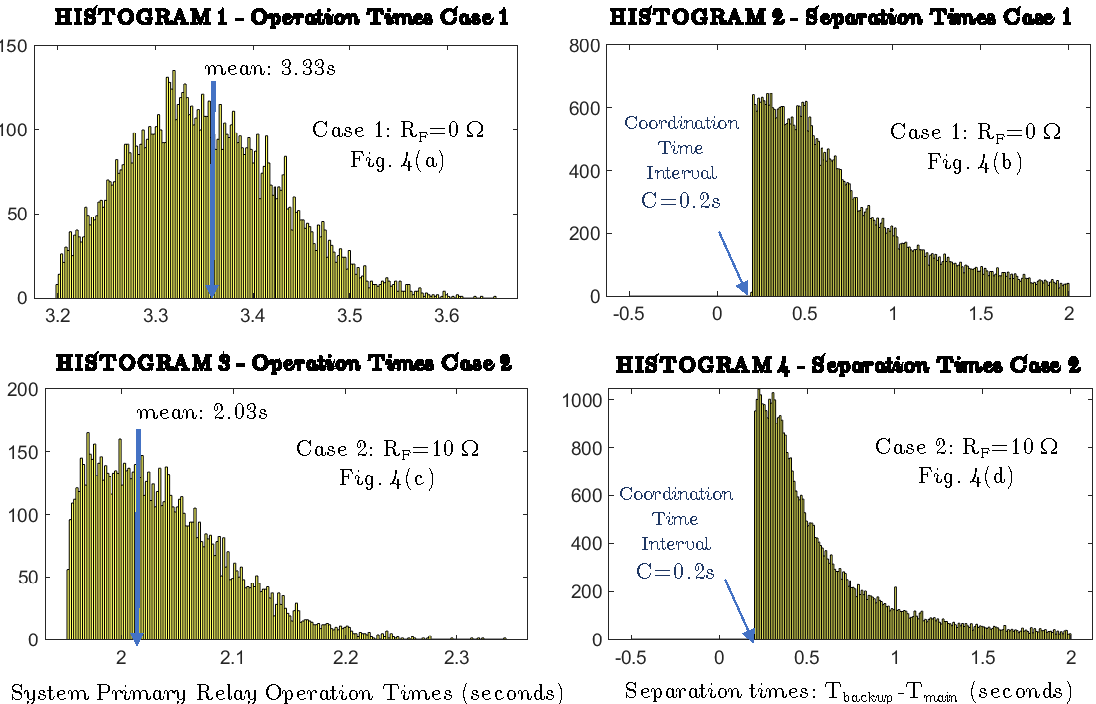
\includegraphics[width=7cm]{images/val1.png}}
       \caption{Test system - Verifying selectivity in Case 1}
      \label{figure5x}
        \end{figure}

        Since all separation times are greater than the coordination interval (0.2s). results show that optimal settings ensure 100 \% selectivity for any fault in the system.

\subsection{Case 2: $R_F$ = 10 $\Omega$}\label{2}

 According to Table \ref{kappas2} and the formulation given in Eq. \ref{kappas2}, the resulting optimization model for  a non-solid fault, $R_F$ = 10 $\Omega$  is given by:

\scriptsize
\begin{equation}\nonumber
   \min_{\mathbf{D^*}}\quad 2.01 D_1+2.23   D_2+2.25  D_3+2.17  D_4+ 2.14   D_5+2.67 D_6
\end{equation}

\begin{eqnarray}\nonumber
&&\mbox{subject to}:\\\nonumber
&&  \begin{bmatrix}
-1.99	&	0.00	&	0.00	&	0.00	&	4.18	&	0.00	\\	
3.03	&	0.00	&	-1.99	&	0.00	&	0.00	&	0.00	\\	
0.00	&	0.00	&	3.07	&	0.00	&	-1.99	&	0.00	\\	
16.71	&	0.00	&	-3.07	&	0.00	&	0.00	&	0.00	\\	
0.00	&	-1.99	&	0.00	&	2.89	&	0.00	&	0.00	\\	
0.00	&	0.00	&	0.00	&	-1.99	&	0.00	&	3.46	\\	
0.00	&	3.86	&	0.00	&	0.00	&	0.00	&	-1.99	\\	

  \end{bmatrix}
  \begin{bmatrix} \nonumber
  D_1\\D_2\\D_3\\D_4\\D_5\\D_6\\
  \end{bmatrix}
\ge  \begin{bmatrix} \nonumber
  0.2\\0.2\\0.2\\0.2\\0.2\\0.2\\
  \end{bmatrix}\\\nonumber
& & 0.1\le{D_i}\quad i=1...6\\\nonumber
 \end{eqnarray}
\normalsize

Notice that only seven relays are capable to detect the fault current.  Three rows coordination matrix should be also removed since some backup fault currents are going in the opposite direction and two rows correspond to a negative operation time (see Table \ref{kappas2}).

The optimal clearing time obtained 2.3222s. Notice that this time is lower than the one obtained in previous case 1 and the optimal settings are:
$D_1$=0.1617,
$D_2$=0.1282,
$D_3$=0.1457,
$D_4$=0.1572,
$D_5$=0.1247
, and $D_6$=0.1484. All separation times (given by $\mathbf{B}\cdot \mathbf{D}$ are equal to the prescribed coordination time (0.2s).


As done in case 1 we verify the appropriateness of the optimal settings obtained by simulating 5000 random faults and determining the corresponding separation times. Results of the selectivity simulation are depicted in the histogram shown in Fig. \label{figure6x}. The number of fault currents to be detected is 60000.
The number of detected fault currents is  48909 (81.52 \%). The mean operation times calculated with the resulting optimal time dial settings is  2.0353s with standard deviation
 0.0589.

 \begin{figure}[t!] \centerline{
     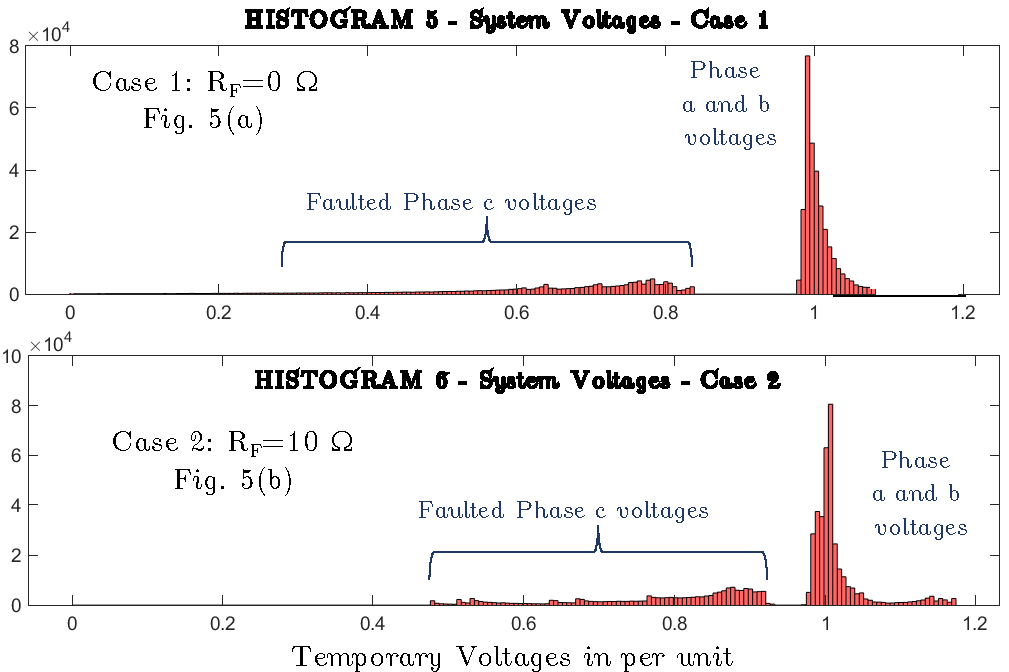
\includegraphics[width=7cm]{images/val2.png}}
       \caption{Test system - Verifying Selectivity in Case 2}
      \label{figure6x}
        \end{figure}


Notice that for a fault of 10 $\Omega$, the objective function is lower than the one obtained for solid faults. In few words, speed associated with settings of case 2 with $R_F$=10 $\Omega$ is faster than speed associated with settings of case 1 with $R_F$=0  $\Omega$. If in real-world the majority of faults have resistance 10 $\Omega$ and the settings are fixed with the traditional approach (solid faults case 1) the actual operation time will not be optimal and far to the best result given by case 2. This result is similar for any fault resistance different than zero.


 \begin{figure}[t!] \centerline{
     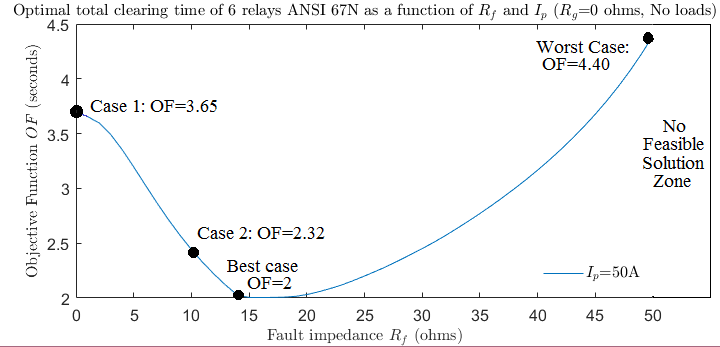
\includegraphics[width=9cm]{images/OF.png}}
       \caption{Test system - Optimal clearing times between $R_F$=0.0 and 50 $\Omega$}
      \label{figure5}
        \end{figure}

         \begin{figure}[t!] \centerline{
     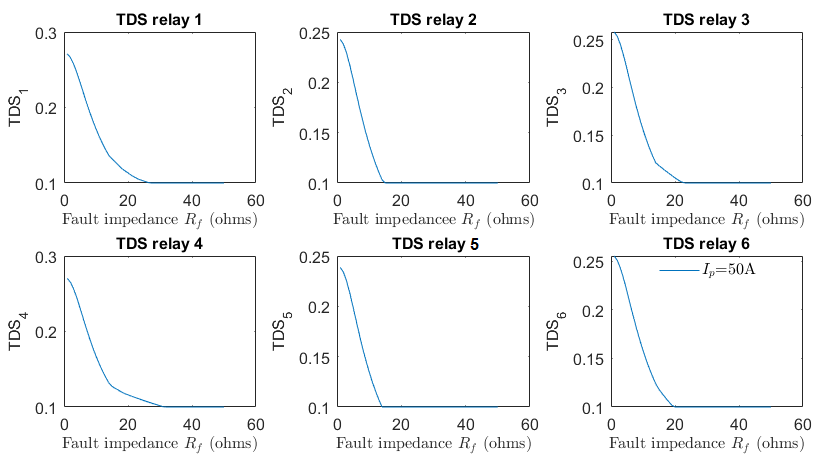
\includegraphics[width=9.0cm]{images/TDS.png}}
       \caption{Test system - Optimal TDS between $R_F$=0.0 and 50 $\Omega$}
      \label{figure6}
        \end{figure}

\subsection{Verification with non-solid faults}\label{s3}

One aspect that we can verify is what happen with speed and selectivity solutions if we setup the TDS of all relays with the optimal settings reported in vase 1 (section \ref{1}, solid faults), but the actual fault magnitude is different than zero as simulated in case 2 (section \ref{2}, $R_F$=10 $\Omega$). In this case, after simulate 5000 random locations for faults with $R_F$=10 $\Omega$ we observe average operational times larger than the optimal ones reported in case 2. In this case, optimal TD settings for solid faults yield a non-optimal solution when the actual fault impedance magnitude is different than zero. However, selectivity is not affected since separation times are greater than the coordination interval in all feasible primary-backup pairs. This result must not be considered a general case and further elaboration is required.

\subsection{Sensitivity analysis }\label{3}

From cases 1 and 2 we observe a decrease on both the objective function and time dial settings. Thus, if the fault impedance is steadily increased we expect to find an impedance value that produce the minimal operation time and the minimal settings allowed (0.1). A sensitivity analysis  was carried out to verify this behavior by producing faults in a range
between 0 and value that makes the optimization problem not well-defined ($R_F$=50  $\Omega$) in steps of 0.1 $\Omega$. Thus, 500 optimization problems were solved. Figure \ref{figure5} and \ref{figure6} displays the OF and the optimal relay time dial settings required to get minimum clearing times, respectively.

 Figure \ref{figure5} depicts the solutions reported in case 1 ($R_F$=0 $\Omega$) and case 2 ($R_F$=10 $\Omega$). The minimum value of the OF is reached when $R_F$=14.9 $\Omega$ (OF = 2.005s). As seen in Fig.  \ref{figure6} this minimum value occurs when $D_2$=$D_5$=0.1.

  If we continue increasing $R_F$ from 15 $\Omega$ to 50 $\Omega$ the OF  steadily increases up to reach a maximum (4.22s for $R_F$=50  $\Omega$) with invariant optimal time dial settings). The fact that optimal time dial settings do not change from 17.5 up to 50 $\Omega$  implies that separation times will increase as far as the fault impedance also increases.  For $R_F>$=50.0  $\Omega$ the optimization problem is not well defined due to sensitivity problems in some relay pairs and no efficient relay coordination is attainable.

\section{Conclusions} \label{conclusions}

In this paper we analyze how optimal operation times and selectivity regarded to optimal coordination of  neutral directional overcurrent relays are affected considering different impedance phase-to-neutral fault magnitudes. Usually optimal coordination has been carried out assuming solid faults. The optimization procedure is performed considering a wide range of fault impedances.

Results show how the optimal operation time decreases as far as the fault impedance magnitude increases. In this process the calculated time dial settings also decreases stagnating at their minimum values. Beyond this point, the time dials are bounded and the clearing times deteriorate as far the fault impedance also increases. In this example, the change of trend, the lowest operation time occurs when the fault impedance is around 15 $\Omega$.

We also find in this example that if the TDSs are specified by the protection engineer considering solid faults but the actual fault type is non-solid, simulations show a non-optimal solution (larger operation times than the ones expected by the optimization problem. This means that current practice based on solid faults may produce suboptimal solutions from operation speed viewpoint.

The main limitation of this work lies on the deterministic representation of the fault resistance. Future work must pose this problem as a stochastic optimization problem. Further efforts would be devoted to solve this problem considering a more realistic condition accounting transient configurations during the clearing time process. In this case, the use of near-end and far-end faults o setup the optimization model should not be enough to assure full selectivity.








 % \scriptsize
%\begin{verbatim}
%clear all
%New circuit.SOURCE_1a bus1=n1.1 bus2=n1.4
%basekV=39.84 pu=1 angle=0    Z1=[0,  9.50] basefreq=60 phase=1
%New Vsource.SOURCE_1b bus1=n1.2 bus2=n1.4
%basekV=39.84 pu=1 angle=-120 Z1=[0,  9.50] phase=1
%New Vsource.SOURCE_1c bus1=n1.3 bus2=n1.4
%basekV=39.84 pu=1 angle=120  Z1=[0,  9.50] phase=1
%New Vsource.SOURCE_2a bus1=n3.1 bus2=n2.4
%basekV=39.84 pu=1 angle=0    Z1=[0, 22.85] phase=1
%New Vsource.SOURCE_2b bus1=n3.2 bus2=n2.4
%basekV=39.84 pu=1 angle=-120 Z1=[0, 22.85] phase=1
%New Vsource.SOURCE_2c bus1=n3.3 bus2=n2.4
%basekV=39.84 pu=1 angle=120  Z1=[0, 22.85] phase=1
%New Vsource.SOURCE_3a bus1=n5.1 bus2=n3.4
%basekV=39.84 pu=1 angle=0    Z1=[0, 17.14] phase=1
%New Vsource.SOURCE_3b bus1=n5.2 bus2=n3.4
%basekV=39.84 pu=1 angle=-120 Z1=[0, 17.14] phase=1
%New Vsource.SOURCE_3c bus1=n5.3 bus2=n3.4
%basekV=39.84 pu=1 angle=120  Z1=[0, 17.14] phase=1
%set earthmodel=carson
%new wiredata.c1 Runits=mi Rac=0.2023 GMRunits=ft GMRac=0.02600
%new wiredata.c2 Runits=mi Rac=0.1756 GMRunits=ft GMRac=0.03210
%new wiredata.n  Runits=mi Rac=0.5920 GMRunits=ft GMRac=0.00814
%!!!! line 1-2
%new linegeometry.4wire12 nconds=4 nphases=3 reduce=no
%~ cond=1 wire=c2 units=ft x=5.5    h=40
%~ cond=2 wire=c2 units=ft x=5.5    h=50.6
%~ cond=3 wire=c2 units=ft x=5.5    h=61.2
%~ cond=4 wire=n  units=ft x=0      h=82.4
%!!!! line 1-3
%new linegeometry.4wire13 nconds=4 nphases=3 reduce=no
%~ cond=1 wire=c1 units=ft x=6    h=40
%~ cond=2 wire=c1 units=ft x=6    h=47.85
%~ cond=3 wire=c1 units=ft x=6    h=55.7
%~ cond=4 wire=n  units=ft x=0    h=71.4
%!!!! line 2-3
%new linegeometry.4wire23 nconds=4 nphases=3 reduce=no
%~ cond=1 wire=c2 units=ft x=5    h=40
%~ cond=2 wire=c2 units=ft x=5    h=49.7
%~ cond=3 wire=c2 units=ft x=5    h=59.4
%~ cond=4 wire=n  units=ft x=0    h=78.8
%new line.line11 geometry=4wire12 length=25
%units=km bus1=n1.1.2.3.4 bus2=n4.1.2.3.4  Rho=100
%new line.line12 geometry=4wire12 length=25
%units=km bus1=n4.1.2.3.4 bus2=n2.1.2.3.4  Rho=100
%new line.line21 geometry=4wire23 length=20
%units=km bus1=n2.1.2.3.4 bus2=n5.1.2.3.4  Rho=100
%new line.line22 geometry=4wire23 length=20
%units=km bus1=n5.1.2.3.4 bus2=n3.1.2.3.4  Rho=100
%new line.line31 geometry=4wire13 length=30
%units=km bus1=n3.1.2.3.4 bus2=n6.1.2.3.4  Rho=100
%new line.line32 geometry=4wire13 length=30
%units=km bus1=n6.1.2.3.4 bus2=n1.1.2.3.4  Rho=100
%!Reactors
%New Reactor.b1 Phases=1 Bus1=n1.4 Bus2=n1.0 R=000 X=0
%New Reactor.b2 Phases=1 Bus1=n2.4 Bus2=n2.0 R=000 X=0
%New Reactor.b3 Phases=1 Bus1=n3.4 Bus2=n3.0 R=000 X=0
%New Reactor.b4 Phases=1 Bus1=n4.4 Bus2=n4.0 R=0.5 X=0
%New Reactor.b5 Phases=1 Bus1=n5.4 Bus2=n5.0 R=0.5 X=0
%New Reactor.b6 Phases=1 Bus1=n6.4 Bus2=n6.0 R=0.5 X=0
%solve
%New fault.1n Bus1=n4.3 Bus2=n4.4 r=0.0001
%!New fault.1n Bus1=n5.3 Bus2=n5.4 r=0.0001
%!New fault.1n Bus1=n6.3 Bus2=n6.4 r=0.0001
%\end{verbatim}
%\normalsize




\bibliographystyle{IEEEtran}
\bibliography{References}



\end{document}
